% figures/tikz/bfs.tex
% Ablaufdiagramm Breitensuche (BFS)
\documentclass[tikz, border=8pt]{standalone}
\usepackage{tikz}
\usetikzlibrary{shapes.geometric, arrows.meta, positioning}

\tikzset{
  startstop/.style = {
    rectangle, rounded corners=8pt, draw=black, thick,
    fill=green!25, minimum width=3.2cm, minimum height=0.9cm,
    font=\small\bfseries, align=center
  },
  process/.style = {
    rectangle, draw=black, thick,
    fill=blue!15, minimum width=3.2cm, minimum height=0.9cm,
    font=\small, align=center
  },
  decision/.style = {
    diamond, draw=black, thick,
    fill=orange!25, minimum width=2.8cm, minimum height=0.9cm,
    inner sep=2pt, font=\small, align=center
  },
  arrow/.style = {->, >=Stealth, thick}
}

\begin{document}
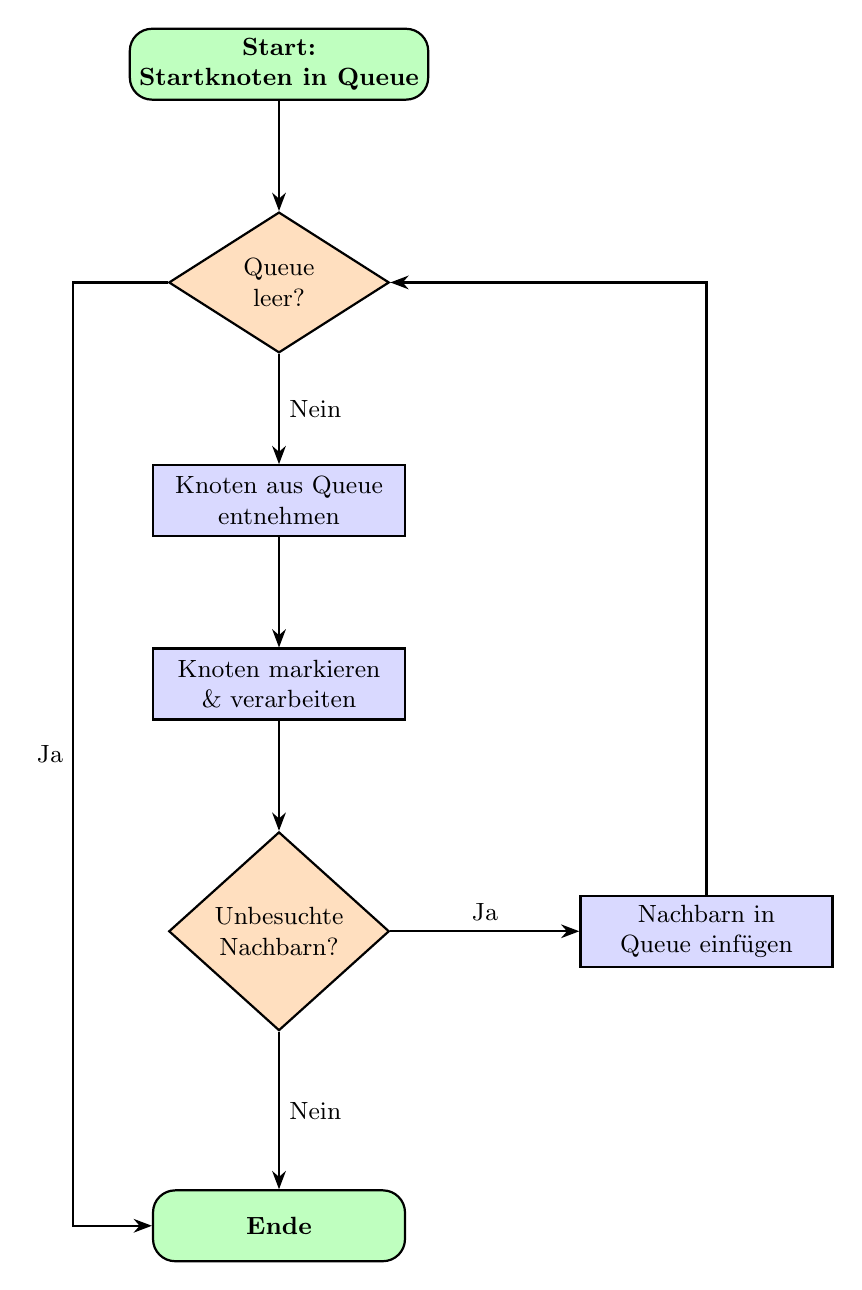
\begin{tikzpicture}[node distance=1.4cm]

  \node[startstop]  (start)  {Start:\\ Startknoten in Queue};
  \node[decision]   (empty)  [below=of start]  {Queue\\leer?};
  \node[process]    (deq)    [below=of empty]  {Knoten aus Queue\\ entnehmen};
  \node[process]    (visit)  [below=of deq]    {Knoten markieren\\ \& verarbeiten};
  \node[decision]   (neigh)  [below=of visit]  {Unbesuchte\\Nachbarn?};
  \node[process]    (enq)    [right=2.4cm of neigh] {Nachbarn in\\ Queue einfügen};
  \node[startstop]  (stop)   [below=2cm of neigh]  {Ende};

  \draw[arrow] (start)  -- (empty);
  \draw[arrow] (empty)  -- node[right]{\small Nein} (deq);
  \draw[arrow] (deq)    -- (visit);
  \draw[arrow] (visit)  -- (neigh);
  \draw[arrow] (neigh)  -- node[above]{\small Ja}  (enq);
  \draw[arrow] (enq)    |- (empty);
  \draw[arrow] (neigh)  -- node[right]{\small Nein} (stop);

  % "Ja"-Rückkante von empty nach stop
  \draw[arrow] (empty.west)
      -- ++(-1.2,0)
      |- node[near start, left]{\small Ja} (stop.west);

\end{tikzpicture}
\end{document}
